A measles epidemic is simulated in a network of affected locations, and vaccine intervention using various resource allocation strategies are implemented in this simulation. These strategies are then compared to gain insight into possible improvements in outbreak response, and to determine whether using UAVs for vaccine deliveries would improve the intervention's success. 

In \S \ref{sec:met_modfr}, a high-level overview of the modelling framework and simulation is presented. This is followed by a full description of the central SEIRVD model employed in the simulation, in \S \ref{meth:MeaslesCompa}. A detailed description of the resource allocation models developed, including team allocations, vaccine delivery allocations, delivery methods, and the DC facility location placement is given in \S \ref{sec:meth_resAlloc}. Metrics for evaluating the success of an intervention are discussed in \S \ref{sec:meth_sim_res}, and details regarding the implementation of the model in the Python programming language are given in \S \ref{sec:meth_softImp}. Finally, \S \ref{sec:res_moVal} concludes the chapter with a validation of the model.

\section{Modelling framework and assumptions}
\label{sec:met_modfr}
For this project, an adapted spatial discrete-time SEIRVD model including vaccinations and deaths is implemented. Discrete time is used in order to link the epidemic model with daily vaccine deliveries across the network. The spatial SEIRVD model spans across a network of connected locations, with a distinct SEIRVD model for each network location. These SEIRVD models are linked by migration, representing the movement of individuals between communities, to form a spatial SEIRVD model. The epidemic model is linked with a resource allocation model through two parameters; the vaccine stock at each network location, and the number of vaccination teams placed at each location. 

A depiction of the general network structure used to model the epidemic over a network of interconnected locations is given in Figure \ref{fig:meth_SEIRschem}; in this case, there are three network nodes. Each node has a certain number of susceptible (S), exposed (E), infectious (I), recovered (R), dead (D) and vaccinated (V) individuals, according to the SEIRVD model -- and each node is connected to each other node through the migration of individuals between them. 

\begin{figure}[ht!]{\textwidth}
    \centering
    \resizebox{0.75\textwidth}{!}{\input{SEIR4nodes.pdf_tex}}
    \caption{Schematic of a simple 3-node network on day $t$, to illustrate epidemic spread through the network.}
    \label{fig:meth_SEIRschem}
\end{figure}

As in all mathematical models, there are assumptions employed in this project. The most significant assumptions are listed below:
\begin{itemize}
    \item There is only a single DC used in the network, with an uncapacitated supply of vaccines that can be delivered to vaccination sites. 
    \item Vaccination teams assigned to the location where the DC is placed, are assumed to have infinite vaccine stock available.
    \item Vaccination teams take no vaccine stock with them to vaccination sites.
    \item There is a single vaccine stockpile per location, shared between the teams at the location.
    \item Vaccines are transported to vaccination sites in cold boxes, entirely outside of the cold chain.
    \item The transportation of diluents and ice are not included in the model.
    \item The population modelled for the epidemic only consists of children under the age of 15.
    \item Vehicle deliveries are performed by two types of vehicle; a primary, larger vehicle, and a smaller vehicle which can traverse rougher terrain. These vehicles have constant capacities.
    \item Roads in the network which are selected to be closed initially, remain closed for the entire simulation, and travel time per road remains constant.
    \item Vaccine deliveries for each day arrive before the vaccines delivered are administered by teams.
    \item Locations are classified as urban if they have good road connections.
    \item Fixed-post teams are sent to urban locations, and mobile teams to rural locations. 
    \item The number of vaccinations per team per day remains constant for the duration of the simulation.
    \item Daily turnout at each location is normally distributed, with a constant mean not depending on the location's population, and not depending on the progression of the epidemic either.
    \item The proportion of each location's population moving to each other location remains constant for each day of the simulation.
    \item Teams reassigned to different locations are immediately available to perform vaccinations on the day that they are reassigned.
\end{itemize}

\section{Epidemic model formulation and notation}
\label{meth:MeaslesCompa}
The SEIR model discussed in \S \ref{sec:lit_SEIR} is adapted to apply to measles and to incorporate Dead (D) and Vaccinated (V) categories, to form an SEIRVD model. Furthermore, spatial dynamics are included by adding a term representing migration to model movement between communities (or between nodes in the context of a network model). 

Let $S_{i,t}$ denote the number of susceptible individuals at location $i \in \{1,\dots,n \}$ at time $t \in \{1,\dots, \mathcal{T} \}$. Similarly, let $E_{i,t}$, $I_{i,t}$, $R_{i,t}$, $V_{i,t}$, and $D_{i,t}$ represent the number of exposed, infectious, recovered, vaccinated and dead individuals at location $i \in \{1,\dots,n \}$ at time $t \in \{1,\dots, \mathcal{T} \}$, respectively. Then, for each network node $i \in \{1, \dots, n\}$ and day $t \in \{1, \dots,\mathcal{T}\}$, the progression of individuals between categories of infection is modelled by the following set of difference equations, which describe the epidemic model entirely:

\begin{align}
S_{i,t+1} &= S_{i,t} - \frac{\beta S_{i,t} I_{i,t}}{N_{i,t}} - v_{i,t} \, \theta^{S}_{i,t} \, \lambda_{S} + \sum_{j=1, j \neq i}^{n} (m_{j,i} S_{j,t} - m_{i,j} S_{i,t}),       \\
E_{i,t+1} &= E_{i,t} + \frac{\beta S_{i,t} I_{i,t}}{N_{i,t}} - \sigma E_{i,t} -  v_{i,t} \, \theta^{E_{72}}_{i,t} \, \lambda_{E} + \sum_{j=1, j \neq i}^{n} (m_{j,i} E_{j,t} - m_{i,j} E_{i,t}), \\
I_{i,t+1} &= I_{i,t} + \sigma E_{i,t} - \gamma I_{i,t} - \mu I_{i,t} + \sum_{j=1, j \neq i}^{n} (m_{j,i} I_{j,t} - m_{i,j} I_{i,t}),   \\
R_{i,t+1} &= R_{i,t} + \gamma I_{i,t} + \sum_{j=1, j \neq i}^{n} (m_{j,i} R_{j,t} - m_{i,j} R_{i,t}),  \\
V_{i,t+1} &= V_{i,t} + v_{i,t} \, \theta^{S}_{i,t} \, \lambda_{S} + v_{i,t} \, \theta^{E_{72}}_{i,t} \, \lambda_{E} + \sum_{j=1, j \neq i}^{n} (m_{j,i} V_{j,t} - m_{i,j} V_{i,t}), \\
D_{i,t+1} &= D_{i,t} + \mu I_{i,t}.
\end{align}

In the above model, $\beta$ denotes the transmission rate of measles, as described in \S \ref{sec:lit_SEIR}, $\sigma$ denotes the proportion of exposed individuals becoming infectious on any given day, $\gamma$ the proportion of infectious individuals becoming recovered, and $\mu$ the proportion of infectious people who die daily. In addition, $m_{i,j}$ denotes the proportion of the population at location $i$ moving to location $j$ daily, and is defined for each pair of locations $i,j \in \{1,\dots,n \}$. 
The number of vaccines administered at location $i$ on day $t$ is denoted by $v_{i,t}$, and $\lambda_{S}$ and $\lambda_{E}$ are the success rates of the measles vaccine in susceptible and recently-exposed individuals (exposed within the preceding 72 hours), respectively. Finally, the susceptible proportion of the remaining unvaccinated population at location $i$ on day $t$ is denoted by $\theta^{S}_{i,t}$, and the recently-exposed proportion by $\theta^{E_{72}}_{i,t}$. Values for $S_{i,t}, E_{i,t}$, $I_{i,t}$, $R_{i,t}$, $V_{i,t}$, and $D_{i,t}$ are rounded up or down probabilistically (randomly, according to how close the value is to its floor and ceiling), to ensure that the values remain whole numbers. 

\subsection{Measles progression parameters} %3.2.1
The parameters that govern the progression of measles through a population include $\beta$, $\sigma$, $\gamma$, $\lambda_{S}$, $\lambda_{E}$, $\theta^{S}_{i,t}$, and $\theta^{E72}_{i,t}$. These are parameters that decision makers have no control over.

After exposure, individuals take an average of 10 days before becoming infectious \cite{moss2007measles}. Therefore, a value of $\sigma = \frac{1}{10}$ is used for the SEIRVD model. Infectious individuals recover after an average of 8 days \cite{who_2019}, so the value used for $\gamma$ is $\frac{1}{8}$.
A value of $R_{0} = 15$ is assumed for the basic reproductive number of measles \cite{guerra2017basic}, corresponding to a transmission rate of $\beta = \frac{15}{8}$. The daily death rate is taken to be $\frac{0.1}{8}$, because individuals are infectious for 8 days, and the death rate per case is assumed to be 10\% \cite{moss2007measles}.

The vaccine success rate in susceptible individuals is assumed to be $\lambda_{S} = 0.95$, since the vaccine is ineffective in 2\% to 5\% of the population, usually \cite{cdc_pinkbook_2018}. The success rate of post-exposure prophylaxis (that is, the success rate of the vaccine in recently-exposed individuals) is taken to be $\lambda_{E} = 0.83$ \cite{csiro_2009}. 

With the number of vaccinations performed on day $t$ at node $i$ denoted by $v_{i,t}$, the susceptible proportion of the remaining unvaccinated population is calculated as
$$\theta^{S}_{i,t} = \frac{S_{i,t}}{S_{i,t}+E_{i,t}+R_{i,t}}.$$ 
This is essentially the probability that any individual arriving to be vaccinated is susceptible, and neither exposed nor recovered.

Individuals that have only been exposed to the measles virus for less than 72 hours can be vaccinated, a practice known as post-exposure prophylaxis. The ratio of recently-exposed individuals to the remaining unvaccinated population of location $i$ on day $t$ is: $$\theta^{E_{72}}_{i,t} = \frac{\sum^{t}_{k=t-3} \frac{\beta S_{i,k}I_{i,k}}{N_{i,k}}}{S_{i,t}+E_{i,t}+R_{i,t}}.$$ 
As before, this is the probability that a vaccine recipient has been exposed to the measles virus within the last 72 hours, has not been exposed for longer, and is neither recovered, nor susceptible.

\subsection{Migration parameters} %3.2.2
\label{sec:meth_migration}
In order to link the distinct compartmental models of all the network's locations, migration of individuals between locations is modelled, using the gravity model of migration. Let $N_{i,t}$ and $N_{j,t}$ be the population values at locations $i$ and $j$ respectively on day $t$, and let $\Delta_{i,j}$ be the distance between the two locations, as calculated in \S \ref{sec:meth_netLoc}. Then, as formulated in Kraemer \textit{et. al} \cite{kraemer2019utilizing}, the total number of people moving from location $i$ to $j$ each day, is
$$T_{i,j,t} = k_{m} \frac{N_{i,t}^{\alpha'} N_{j,t}^{\beta'}}{\Delta_{i,j}^{\gamma'}}.$$ 

The model has parameters $k_{m}, \alpha', \beta',$ and $\gamma'$. The parameter $k_{m}$ is an adjustable multiplier in the model, representing the frequency of migration. This can be used in sensitivity analysis to test the effect of changes in migration on the progression of the epidemic. 

The values of $\alpha'$ and $\beta'$ govern the importance of each location's population on the migration between them; there are more people moving daily between two nearby cities than two nearby villages. For simplicity, these are assumed to be equal, with $\alpha' = 0.5$, and $\beta' = 0.5$. This means that both locations' populations have an equal effect on the amount of migration. Since $\alpha' + \beta' = 1$, this gravity model is similar to the radiation model of migration with uniform population density \cite{simini2012universal}. The latter can unfortunately not be implemented due to the lack of census data for the network, although it often offers more accurate results. 

Finally, the $\gamma'$ parameter incorporates the distance between locations into the model; the higher the value of $\gamma'$, the larger the impact of distance on migration. Intuitively, the further apart two locations are, the fewer people move between the two daily. This value is dependent on terrain and is location-specific. If $\gamma' = 2$ is used, the model corresponds with Newton's law of gravity, although values below this are also commonly used \cite{poot_alimi_cameron_maré_2016}. For the sake of generality, a value of $\gamma' = 2$ is used for the model. 

Note that $T_{i,j,t}$ must be discrete; so the value is rounded up or down to its \textit{ceiling} or \textit{floor} probabilistically, according to how close the value is to each of the two. Due to this random daily rounding in migration numbers, $N_{i,t} \text{ and } N_{j,t}$ fluctuate. However, these fluctuations are so small they can be considered negligible. Further, if deaths were to occur and the population reduces as a result, the proportion of the population migrating to certain locations over other locations would not change significantly. Thus, to simplify notation, let $N_{i,t} = N_{i}$, and $T_{i,j,t} = T_{i,j}, \, \forall{i,j} \in \{1,\dots,n\}$. With this simplification, and the aforementioned assumed parameter values used, the equation simplifies to:
$$T_{i,j} = k_{m} \frac{\sqrt{N_{i} N_{j}}}{\Delta_{i,j}^{2}}.$$

Now, since each location has a distinct SEIRVD model, the total number $T_{i,j}$ of migrations between $i$ and $j$ is comprised of people in each of the S, E, I, R, and V categories. Naturally, there is no migration for deceased individuals in the D category. In order to implement this division of migration between categories, a proportion $m_{i,j}$ is calculated. This is the proportion of people in location $i$ which migrate to location $j$, daily: $$m_{i,j} = \frac{T_{i,j}}{N_{i}}.$$ Because $N_{i}$ and $T_{i,j}$ remain constant over time, this proportion is also constant. So, for each $i \in [1,\dots,n]$ and $j \in [1,\dots,n]$, $m_{i,j}$ is set to be the (i,j)-th entry in a matrix of constant migration proportions, used in equations (3.1)-(3.6). This matrix of migration proportions is calculated before the simulation begins, and is held constant throughout.

\subsection{Number of vaccinations} %3.2.3
\label{sec:meth_numVaccs}
Each location $i$ hosts a number $\eta_{i,t}$ of vaccination teams (on each day $t \in \{1,\dots \mathcal{T} \}$), as assigned for a given day. The number of people each team in location $i$ can vaccinate daily is assumed to be $\psi_{i} = 450$ if the team is a fixed-post team, and $\psi_{i} = 250$ if the team is mobile. It is assumed that fixed-post teams are deployed in urban areas, and mobile teams in rural areas. Thus, the maximum number of vaccinations that all the teams in area $i$ can perform daily is $\psi_{i} \,\eta_{i,t}$. 
The number of vaccinations which can occur daily in a location also depends on the day's turnout for vaccinations $\tau_{i,t}$, as well as the number of vaccines available there, $\nu_{i,t}$.  
The day's turnout is randomly generated according to the normal distribution, with a mean of $\Bar{\tau}_{i,t} = 450$ for rural areas, and $\Bar{\tau}_{i,t} = 900$ for urban areas. An approximated variance of $\sigma^2_{\tau} = \frac{1}{5} \Bar{\tau_{i,t}}$ is used to obtain a reasonable spread of values. Turnout only includes susceptible, exposed and recovered members of the population; infected, dead and already-vaccinated individuals are not vaccinated. Exposed individuals would not be aware that they are exposed, as symptoms of measles only appear once infectious. Vaccination teams often vaccinate people non-selectively, being unaware whether a recipient is already immune, susceptible or exposed. Non-selective vaccination is sometimes used in outbreak response where there is a very high risk of the epidemic spreading \cite{danet_fermon_2013}, which is indeed the case for measles outbreaks. By placing all individuals assumed to have been vaccinated previously in the V class instead of the R class in the model input, vaccination can be targeted to those individuals actually requiring vaccines. This does have the limitation that documentation regarding previous vaccinations needs to be checked, but due to the short time period modelled in the simulation, it is unlikely that a vaccinated individual would return for another vaccination, and so, targeted vaccination is assumed.

Combining all of the aforementioned limits on vaccinations, the number of vaccinations occurring at location $i$ on day $t$ is 
$$v_{i,t} = \text{min} \{\psi_{i} \,\eta_{i,t}, \tau_{i,t}, \nu_{i,t} \}.$$ 

Both $\eta_{i,t}$ and $\nu_{i,t}$ are determined by decision-makers, and are therefore used as the decision variables in the resource allocation models formulated in \S \ref{sec:meth_resAlloc}.

\subsection{Network structure} %3.2.4
\label{sec:meth_netLoc}
The epidemic simulation requires an input dataset containing information about a physical network of locations, and the size of the population in each location. For the sake of generality, let the number of locations be $n$. A measles outbreak may then be simulated on this given network to study the effectiveness of UAV vaccine delivery, and compare resource allocation strategies. 

As input, the model requires each of the following values for each location in the network:
\begin{itemize}
    \item Name -- for better reporting of results, each location must be assigned a name.
    \item Urban -- a true/false value indicating whether the location is urban or not. Locations with good road connections and large populations are assumed to be urban.
    \item x$_{i}$ -- the scaled Euclidean x-coordinate of the location. Location coordinates are scaled such that the calculated Euclidean distance between any pair of locations is near to the actual distance between those locations in the physical network.
    \item y$_{i}$ -- the scaled Euclidean y-coordinate of the location.
    \item $N_{i,t}$ -- the number of children under the age of 15 residing in the location (or, for more general epidemic models, the number of individuals possibly affected by the epidemic).
    \item $S_{i,t}$ -- the number of susceptible individuals at the start of the simulation, at this location.
    \item $E_{i,t}$ -- the number of exposed individuals at the start of the simulation, at this location.
    \item $I_{i,t}$ -- the number of infectious individuals at the start of the simulation, at this location.
    \item $R_{i,t}$ -- the number of recovered individuals at the start of the simulation, at this location. Previously-vaccinated individuals can be included in this category if vaccination is untargeted; then, individuals are vaccinated regardless of their prior vaccination status.
    \item $V_{i,t}$ -- the number of vaccinated individuals at the start of the simulation, at this location. Previously-vaccinated individuals can be included in this category if vaccination is targeted.
    \item \textit{mapX}$_{i}$ -- the x-coordinate of the location for use in visually plotting the network programmatically.
    \item \textit{mapY}$_{i}$ -- the y-coordinate of the location for use in visually plotting the network programmatically.
\end{itemize}

This input data for the model can be represented in a table, with each described attribute linked to each location. Additionally, road distances between locations are required as input for the simulation; direct distances between each pair of locations by road can be supplied in the form of a table. If there is no direct road between two locations, that road distance can simply be left blank.

\subsection{Initial conditions} %3.2.5
The input data required for the model includes initial values for $N_{i,0}$, $S_{i,0}$, $E_{i,0}$, $I_{i,0}$, $R_{i,0}$, and $V_{i,0}$, for each location $i \in \{1,\dots,n\}$. These values are set to the input values supplied. 
In the input data, $E_{i,0}$, $I_{i,0}$, and $D_{i,0}$ are set to zero for all locations, except for some index cases specified in a location selected to be the epicentre of the epidemic. Index cases are represented by setting $I_{i,0}$ to the number of initial infectious individuals in the epicentre.

Once the input data for the network is entered into the model, the distance between locations $i$ (at coordinates $(x_{i},y_{i})$) and $j$ (at coordinates $(x_{j},y_{j})$) is calculated. This distance is calculated as the Euclidean distance between the locations: 
$$\Delta_{i,j} = \sqrt{(x_{i} - x_{j})^{2} + (y_{i} - y_{j})^{2}}\,, \qquad \forall{ i \in 1,\ldots,n},\quad \forall{ j \in 1,\ldots,n}.$$ 

Migration proportions $m_{i,j}$ are calculated initially and held constant for the duration of the simulation, and vaccine stock $\nu_{i,0}$ at each location $i \in \{1,\dots,n\}$ is set to zero at first. Teams are assigned on each day of the simulation, so there is no need for an initial value of $\nu_{i,t}$ as it'll be assigned on the first day by the resource allocation model. 

\section{Resource allocation models} %3.3
\label{sec:meth_resAlloc}
The epidemic model formulated in \S \ref{meth:MeaslesCompa} indirectly depends upon certain parameters which can be controlled by decision makers. More specifically, the parameter in the SEIRVD model defined that decision makers have control over is the number of vaccinations performed at each location daily, $v_{i,t}$. Recall that the number of vaccinations $v_{i,t}$ is constrained by the number of vaccination teams at location $i$, $\eta_{i,t}$, and the number of vaccines in stock, $\nu_{i,t}$, as well as turnout. Only $\eta_{i,t}$ and $\nu_{i,t}$ are considered in this project as decision variables in the resource allocation models. While decision makers can have some impact on turnout through awareness campaigns, they do not have direct control over turnout. Both $\eta_{i,t}$ and $\nu_{i,t}$ can be determined using resource allocation models for team allocation and vaccine delivery scheduling, respectively. Additionally, vaccine deliveries depend upon the location selected as the distribution centre of the network, and the vaccine delivery method selected. 

A discussion of the method used for placement of the distribution centre is given in \S \ref{sec:res_DCloc}. 
This is followed by a description of various team allocation methods in \S \ref{sec:team_strat}, and vaccine allocation methods in \S \ref{sec:vd_strat}. Team allocations influence the SEIRVD model by directly affecting $v_{i,t}$. Vaccine allocations, on the other hand, select locations to receive vaccine stock, which affects $v_{i,t}$ through $\nu_{i,t}$. Delivery of vaccines to the locations selected is performed by the vaccine delivery methods described in \S \ref{sec:dro_dels} and \S \ref{sec:veh_dels}; either by UAV, vehicle, or both UAVs and vehicles.

\subsection{DC location placement} 
\label{sec:res_DCloc}
In a network in which a measles outbreak occurs, when vaccination teams are placed at locations in the network, a central DC is needed as a centre of operations for the teams, and for refrigerated vaccine storage. In a UAV delivery network, the DC would also have equipment for the launching, tracking and landing of the UAVs used. This DC would need stable electricity access and good road connections (in order for large quantities of vaccines to be delivered to it by truck or car), so therefore must be placed in an urban area.

The objective of this DC placement is to select an urban location, such that as many other locations as possible are within the flight range of the UAVs, if a UAV delivery network is used. The flight range of the Zipline UAVs considered in this project is 160km \cite{czerwonka_2018,service_contract_2018,zipline_impact}, so all locations need to be within 80km of the DC, if possible. This problem is of a static nature, independent of the progression of the epidemic, and is therefore solved before the simulation of the epidemic begins. Other methods could potentially be used which incorporate population sizes, but for the sake of simplicity, population sizes are disregarded for this problem. The assumption that only one DC is required as a flight base to cover the network simplifies the placement problem significantly -- the objective is now to select a location from those in the network having electricity access, such that as many other locations as possible are less than 80km from the selected location. 
This is equivalent to choosing a feasible location $i^{*}$, such that the maximum distance from $i^{*}$ to any other location $j \neq i^{*}$, is minimized. This is a simplified version of the minimax multifacility location problem with euclidean distances formulated by Elzinga, Hearn and Randolph \cite{elzinga_1976}. Since the problem uses no fixed value for UAV flight range anywhere, it can be applied to cases where other UAVs are used.
More formally, where $(i'_{1},\ldots,i'_{n'})$ are the locations from $(1,\dots,n)$ having electricity access, the DC is placed at
$$i^{*} = \text{min}_{i'_{1},\ldots,i'_{n'}} \, \text{max} \{\Delta_{i,j}, \, i \in \{i'_{1},\ldots,i'_{n'}\}, \, j \in \{1,\ldots,n\}\}.$$

\subsection{Team allocation model} %3.3.2
\label{sec:team_strat}
Once a measles outbreak intervention begins, a major decision that needs to be made immediately is where to send vaccination teams first. Teams could vaccinate people preemptively before the epidemic reaches their location, or alternatively teams could focus on administering post-exposure vaccinations and treatment to locations where the epidemic is most severe. A combination of these can even be employed. Since the number of deaths resulting from the epidemic is directly proportional to the number of exposures to measles, in order to minimise deaths, a resource allocation model that minimises the number of exposures will indirectly minimise the number of deaths. Therefore, an integer program is developed as a resource allocation model for team allocations, with the objective of maximising expected prevented exposures (EPE) by allocating teams to locations most in need of vaccination teams. 

\subsubsection{Expected prevented exposures allocation strategy}
\label{meth:teamEPE}
Assuming that there are $\mathcal{N}$ vaccination teams to be allocated in the network on day $t$, a number $\eta_{i,t}$ of teams needs to be allocated to each location $i \in \{1, \dots, n\}$, such that $\sum_{i=1}^{n} \eta_{i,t} = \mathcal{N}, \, \forall{t} \in \{1, \dots, \mathcal{T}\}$.  Recall that $\psi_{i}$ denotes the number of vaccinations per team per day at location $i$, $\tau_{i,t}$ is the turnout, and $\nu_{i,t}$ is the number of vaccines in stock. With $\eta_{i,t}$ teams assigned, the number of vaccinations possible will be: $$v_{\eta_{i,t},i,t}  = \text{min} \{\psi_{i} \,\eta_{i,t}, \tau_{i,t}, \, \nu_{i,t} \}.$$ 

Let the number of susceptible individuals remaining after vaccination at location $i$ on day $t$ (but before migration and epidemic progression on day $t+1$) be $$S'_{i,t} = S_{i,t} - v_{\eta_{i,t},i,t} \, \theta^{S}_{i,t} \, \lambda_{S}.$$
Then, with new exposures, prophylaxis administered and progression into the Infectious category taken into account, the expected exposures at location $i$ on day $t+1$ is $$E'_{\eta_{i,t},i,t+1} = E_{i,t} + \frac{\beta S'_{i,t} I_{i,t}}{N_{i,t}} - \sigma E_{i,t} - v_{\eta_{i,t},i,t} \, \theta^{E_{72}}_{i,t} \, \lambda_{E}.$$
Now, for each location $i \in \{1,\dots,n\}$, and each number of teams $\eta_{i,t} \in \{1,\dots \mathcal{N}\}$ that could possibly be assigned to that location, the EPE resulting from that team assignment is calculated:
$$E^{*}_{\eta_{i,t},i,t+1} = E'_{0,i,t+1} - E'_{\eta_{i,t},i,t+1}, \quad \forall{i} \in \{1, \dots, n \}, \text{ and } \forall{\eta_{i,t}} \in \{1,\dots \mathcal{N} \}.$$

A knapsack problem is formulated with the objective of maximising total EPE by allocating teams to locations which need teams the most. This knapsack problem is to
\begin{align}
\label{eqn:EPEteams}
    \text{maximise\quad} & \sum^{n}_{i=1} E^{*}_{\eta_{i,t},i,t+1} \\ 
    \text{s.t.\qquad} & \sum^{n}_{i=1} \eta_{i,t} \leq \mathcal{N}, \\
    &\eta_{1,t}, \eta_{2,t}, \ldots, \eta_{n,t} \text{ integer}.
\end{align}

Constraint (3.8) ensures that the number of teams allocated in the network does not exceed the total number of teams available, $\mathcal{N}$. Constraint (3.9) ensures that the team assignment found has integer values for teams.

\subsubsection{Solution approach}
This knapsack problem is solved by iteratively assigning one team at a time to the location with the highest increase in EPE resulting from the newly-added team. This way, the greatest ratio of payoff (EPE) to cost (using one of the available teams) is selected repeatedly, until there are no teams remaining.
Note that any integer knapsack problem can be reformulated as a 0/1 knapsack problem \cite[p.~150]{winston2004operations}, and when (3.7) is reformulated as such, this greedy solution procedure is akin to the branch and bound method used by Winston and Goldberg for solving 0/1 knapsack problems -- which produces an optimal solution when the constraint is binding (i.e. when all teams are assigned, which is always the case here) \cite{avis_2002}. 

Initially, $\eta_{i,t} = 0, \, \forall{i} \in \{1,\dots,n \}$.
Then, the first team is allocated to the location $$i' = \text{max}_{i} \left\{ \frac{E^{*}_{(\eta_{i,t}\,+\,1),i,t+1}}{(\eta_{i,t} + 1)}, i \in \{1, \dots, n\} \right\},$$ 
by incrementing $\eta_{i',t}$ such that $\eta_{i',t} = 1$. The second team is allocated in the same manner, with the only difference being that $\eta_{i',t} = 1$ instead of zero. This procedure is repeated until there are no more teams remaining to be assigned.

Note that this knapsack problem applies specifically to day $t$, and is solved dynamically for each day $t \in \{1, \dots, \mathcal{T} \}$ in the simulation.

\subsubsection{Heuristic strategies for team allocation}
The objective of any team allocation strategy in epidemic response is to minimise the number of deaths caused by the epidemic and curb the spread of the epidemic. This is equivalent to minimising expected prevented exposures. However, most intuitive team allocation strategies do not solve the resource allocation model in (\ref{eqn:EPEteams}) optimally, and they can be considered as heuristics. Certain intuitive team allocation heuristics are presented below, with teams allocated proportionally to certain location-specific values, and each calculated $\eta_{i,t}$ value rounded up or down probabilistically. These heuristics include:

\begin{itemize}
    \item Population (N) -- the number of teams allocated to each location is proportional to the location's population: $$\eta_{i,t} \simeq \mathcal{N} \times \frac{N_{i,t}}{\sum_{j=1}^{n} N_{j,t}}.$$
    \item Susceptible (S) -- the number of teams allocated to each location is proportional to the number of susceptible, unvaccinated people in that location: $$\eta_{i,t} \simeq \mathcal{N} \times \frac{S_{i,t}}{\sum_{j=1}^{n} S_{j,t}}.$$
    \item Infections (I) -- the number of teams allocated to each location is proportional to the number of currently infected individuals in the location: $$\eta_{i,t} \simeq \mathcal{N} \times \frac{I_{i,t}}{\sum_{j=1}^{n} I_{j,t}}.$$
    \item Infections Ratio (I/N) -- the number of teams allocated to each location is proportional to the infection ratio of that location (the ratio of infected people to population): $$\eta_{i,t} \simeq \mathcal{N} \times \frac{\frac{I_{i,t}}{N_{i,t}}}{\sum_{j=1}^{n} \frac{I_{j,t}}{N_{j,t}}}.$$
    \item Spread -- one team is allocated to each location in the network (assuming $\mathcal{N} >= n$). If there are extra teams unallocated thereafter, the remaining teams are randomly distributed through the network (note again that these values of $\eta_{i,t}$ are randomly rounded up or down while ensuring that $\sum_{i=1}^{n} \eta_{i,t} = \mathcal{N}$). This results in the following team allocation:
    $$\eta_{i,t} \simeq 1 + \frac{\mathcal{N} - n}{\mathcal{N}}.$$
\end{itemize}


\subsection{UAV vaccine allocation models} 
\label{sec:vd_strat}
The number of vaccines on hand at location $i$ on day $t$, $\nu_{i,t}$, depends entirely on the vaccine delivery schedule modelled. As more vaccines are delivered to location $i$, $\nu_{i,t}$ increases. The greatest challenge is thus to select which locations to deliver vaccines to first, in order to minimise the number of deaths resulting from the measles epidemic. Note again that a resource allocation model which maximises EPE indirectly minimises deaths. Therefore, a knapsack problem similar to the problem in \S \ref{meth:teamEPE} is formulated; maximising EPE per minute of delivery time.

Vaccines can only be delivered to locations where vaccination teams have been sent. Further, since mono-dose measles vaccines can remain potent for 3 days after removal from the cold chain \cite{msf_ectc_2018}, it is assumed that vaccines are delivered in vaccine carriers of various sizes (depending on the delivery method), and that they expire 3 days after delivery. For clarity, the vaccine is assumed to only be reconstituted when it is administered to a recipient, and not any earlier.

\subsubsection{Number of vaccines required}
In order to prevent vaccine wastage, only enough vaccines for the following 3 days are delivered to each location. This is due to the aforementioned assumption that measles vaccines lose potency after 3 days \cite{msf_ectc_2018}. The number of vaccines required for the next 3 days is naturally not known exactly in advance, but is estimated according to expected turnout, team capability, vaccine stock on hand and the number of remaining unvaccinated people in that location. More formally, the (non-negative) number of vaccines still `required' on day $t$ at location $i$, is 
$$v'_{i,t} = \text{max} \left\{ \text{min} \{S_{i,t} + E_{i,t} + R_{i,t}, \, 3 \psi_{i} \eta_{i,t}, \, 3 \bar{\tau_{i,t}} \eta_{i,t} \} - \nu_{i,t}, 0\right\}$$

\subsubsection{Expected prevented exposures strategy}
\label{sec:meth_EPE_strat}
Consider a resource allocation strategy where the objective is to maximise total expected prevented exposures (EPE) to measles per day, by delivering vaccines to the right locations, first.

Let the number of expected exposures on day $t+1$ at location $i$, given that $x_{i}$ vaccines are delivered, be denoted by $E'_{x_{i},i,t+1}$. If $x_{i}$ vaccines are delivered to location $i$ during day $t$, the number of vaccinations possible on day $t$ becomes $$v_{x_{i},i,t} = \text{min} \{\psi_{i} \,\eta_{i,t}, \tau_{i,t}, \, \nu_{i,t} + x_{i} \}.$$ 
The number of expected exposures on day $t+1$ is calculated using the number of susceptible individuals, after vaccination on day $t$ is complete (using the updated $v_{x_{i},i,t}$ value), but before migration and epidemic progression for day $t+1$. This number of susceptible individuals is denoted by $S'_{i,t}$. 
Formally, after vaccinations, the number of susceptible individuals at location $i$ on day $t$ is: $$S'_{i,t} = S_{i,t} - v_{x_{i},i,t} \, \theta^{S}_{i,t} \, \lambda_{S}.$$

Taking $S'_{i,t}$ and the $x_{i}$ vaccines delivered into account, expected exposures on day $t+1$ at location $i$ is given by 
$$E'_{x_{i},i,t+1} = E_{i,t} + \frac{\beta S'_{i,t} I_{i,t}}{N_{i,t}} - \sigma E_{i,t} - v_{x_{i},i,t} \, \theta^{E_{72}}_{i,t} \, \lambda_{E}.$$
Given this value of $E'_{x_{i},i,t+1}$ for expected exposures, the expected prevented exposures due to a delivery of $x_{i}$ vaccines is:
$$E^{*}_{x,i,t+1} = E'_{0,i,t+1} - E'_{x_{i},i,t+1}, \quad \forall{i} \in \{1, \dots, n \}.$$

Let the total time required per delivery to location $i$ be denoted by $\delta_{i}$. Let $d_{i}$ denote the number of deliveries to location $i$ on the day considered. Naturally, if $d_{i}$ increases, $x_{i}$ increases proportionally, depending on the capacity $c$ of the delivery method. Therefore, $x_{i} = c \, d_{i}$.
Then, the allocation of vaccine deliveries to locations that maximises the total number of expected prevented exposures, can be found by solving the following integer program:
\begin{align}
    \text{maximise\quad} & \sum_{i=1}^{n} E^{*}_{x_{i},i,t+1}, \\
    \text{s.t.\qquad} & \sum_{i=1}^{n} d_{i}\,\delta_{i} \leq \mathcal{H}, \\
    &x_{i} \leq v'_{i,t} + c - 1, \quad \forall{i} \in \{1, \dots,n \},\\
    &d_{1}, d_{2}, \ldots, d_{n} \text{ integer}.
\end{align}

Constraint (3.11) ensures that the total amount of delivery time available per day, $\mathcal{H}$, is not exceeded, and constraint (3.12) ensures that the amount of vaccines delivered to each location does not significantly exceed the amount of vaccines needed there, $v'_{i,t}$. Finally, constraint (3.13) simply ensures that the number of deliveries to each location is an integer.
This integer program can be solved by iteratively assigning one more delivery to a location (incrementing one $d_{i}$), where the location $i$ to be delivered to has the highest EPE per minute of delivery time. Essentially, the highest payoff (EPE) per unit of cost (time) is repeatedly selected. This is similar to the branch and bound method used for team allocation and used by Winston and Goldberg in general to solve knapsack problems \cite{winston2004operations}. This solution procedure can be implemented in the simulation by iteratively performing daily deliveries to locations with the highest value of EPE per minute of delivery time. Once a delivery is made, stock levels are updated, the EPE value is recalculated for that location, and the next best location is selected to receive the next delivery. However, unlike the team allocation case, the solution is not necessarily optimal since constraint (3.11) is not always binding.

\subsubsection{Heuristic strategies for vaccine allocation}
\label{sec:meth_delAccHeur}
With the linear program developed in \S \ref{sec:meth_EPE_strat} considered, the objective of vaccine delivery allocation is to maximise the number of expected prevented exposures resulting from each delivery allocated. Three intuitive, more easily implemented strategies of vaccine allocation are defined below, which can essentially be considered as heuristic approaches to solving the linear program to maximise EPE:

\begin{itemize}
    \item Population ($N$) -- vaccines are delivered to locations with the highest population, first. After a sufficient number of vaccines have been delivered, the location or route with the second-highest population is delivered to. The determination of what counts as a sufficient number of vaccines can depend upon the number of days of vaccine potency before expiry. This heuristic solves the LP by incrementing $d_{i}$ until location $i$ has sufficient vaccine stock, where $i$ is the location with the highest population. Thereafter, $d_{i'}$ is incremented, where $i'$ has the second-highest population, and so on.
    \item Susceptible ($S$) -- the location or route with the highest number of susceptible, unvaccinated individuals is delivered to, first. Again, the number of vaccines delivered per location will not exceed the expected number of vaccines required. This heuristic increments $d_{i}$ in the same manner as the $N$ strategy, just considering the number of susceptible individuals instead of population.
    \item Infections ($I$) -- the location or route with the highest number of infectious individuals is delivered to first, in the same manner as the previous two strategies, considering the number of infectious individuals instead of the population.
\end{itemize}

\subsubsection{Time required per delivery}
\label{sec:dro_dels}
The total travel time for a delivery to location $i$ is denoted by $\delta_{i}$.
The direct distance $\Delta_{i,j}$ between locations $i$ and $j$ is used for UAV deliveries instead of the distance by road, because UAV flight paths are not constrained by roads. Thus, assuming the average flight speed is 100km/h \cite{service_contract_2018, zipline_impact}, and the setup time per flight is 10 minutes \cite{ackerman_koziol_2019}, the one-way flight time (in minutes) from the DC ($i^{*}$) to each location $i$ is calculated to be $$\delta_{i} = 10 + \frac{\Delta_{i,i^{*}}}{100} \times 60, \quad \forall{i} \in \{1, \dots, n \}$$ 

\subsubsection{Number of vaccines per delivery}
The UAVs considered have a maximum payload of 1.75kg \cite{service_contract_2018, zipline_impact}. Small vaccine carriers are often used for ``small, one-day immunization outreach sessions," and vaccine transport \cite{unicef_Apex}, and are therefore appropriate for UAV deliveries. The Apex AIDVC-24 small vaccine carrier has a vaccine storage capacity of 0.9$\ell$, and a fully loaded weight of 2.27kg, including two ice packs of 0.4$\ell$ volume \cite{who_carriers_2011}. Thus, without the ice packs, the vaccine carrier's weight is well below the UAV's maximum payload, and can be used. Taking into account the packed volume per measles vaccine dose of 15m$\ell$ \cite{cdc_pinkbook_2018}, and the carrier's vaccine storage capacity of 0.9$\ell$, each carrier can contain 60 vaccine doses. Thus, 60 doses are delivered per UAV flight, and $c=60$ in this case. All deliveries are to single locations; since the UAV considered drops deliveries by parachute, deliveries to multiple locations in a single route are not possible. However, the possibility of multiple simultaneous UAV flights is allowed; different UAVs (the number of which is specified, with an initial value of 2) can be launched in staggered 5-minute intervals -- due to the assumption that there is only a single launching contraption at the DC.

\subsubsection{Solution approach}
The UAV deliveries to be scheduled for a day depend on the vaccine delivery strategy selected. 
If the optimal EPE strategy is used, the number of vaccines delivered is directly proportional to the number of UAV deliveries: $x_{i} = 60 \, d_{i}$. Then, let the location for which the maximum EPE per minute of delivery time is attained be denoted by $$i' = \text{max}_{i} \left\{ \frac{E^{*}_{60,i,t+1}}{\delta_{i}}, i \in \{1, \dots, n\} \right\}.$$ 
This location $i'$ is thus selected to receive the first UAV delivery of the day, according to the solution procedure outlined in \S \ref{sec:meth_EPE_strat}. After the delivery is performed, the EPE value for location $i'$ is recalculated, using the new stock level at location $i'$, and a new location is found which maximises EPE per minute of delivery time.

Alternatively, if the selected delivery strategy is population, then the location $i'$ with the highest value of $N_{i',t}$ per minute of delivery time is selected. Formally, the location selected for the first delivery is $$i' = \text{max}_{i}\left\{ \frac{N_{i,t}}{\delta_{i}}, \, i \in \{1, \dots, n \} \right\}.$$ 
This same method is used for selecting deliveries according to the S and I strategies also.

Regardless of the delivery strategy, the selected location must satisfy the following requirements, otherwise the next best location is selected:
\begin{itemize}
    \item The location selected to be delivered to must not be the DC's location ($i^{*})$. Thus, $i' \neq i^{*}.$
    \item The location selected must actually require a vaccine delivery. If there are no teams at the selected location or there is sufficient stock there already ($v'_{i,t} = 0$), there is no need for a delivery.
    \item Finally, the selected location must not be too far away and not take too long to deliver to; the UAVs must always return before the day's working hours, $\mathcal{H}$, have been completed. If the current time of day for UAV $u$ (in minutes since the working day began) is $t_{\text{mins},u}$, then $t_{\text{mins},u} + \delta_{i'} \leq \mathcal{H}$ is the time constraint.
\end{itemize}

Once a location $i'$ has been chosen that satisfies the above requirements, it is scheduled as a delivery for the day. Since 60 vaccines are delivered per UAV, the vaccine stock on hand at location $i'$ becomes $\nu_{i'} = \nu_{i'} + 60$, and the time of day for UAV $u$ is updated to $t_{\text{mins},u} = t_{\text{mins},u} + \delta_{i'}$. The `time of day' is maintained for each available UAV; it represents the time at which the UAV returns from its current delivery. This allows multiple UAVs to run simultaneously, each having a different delivery schedule. If both UAVs are performing a delivery, the first one to return is immediately sent for the next delivery, and so on. The EPE strategy can still be implemented in the case of multiple UAVs, with locations selected in the same manner.

\subsection{Vaccine allocation model for land-based delivery} 
\label{sec:veh_dels}
Unlike the UAV delivery network, vehicle deliveries are constrained by road networks. This can be a significant constraint when roads are of poor quality and perhaps even nonexistent. For the sake of generality, the average travelling speed and vehicle type are varied depending on the estimated road quality on a route. 

\subsubsection{Determination of impassable roads and land-based delivery times}
Roads are randomly assumed to be passable or not according to probabilities; and roads set as impassable are assumed to remain impassable for the duration of the simulation. The probability of a road being passable is divided by an adjustable multiplier $\mathcal{K}$, initially set to 1. There are multiple cases for which this probability and the average road speed is varied:

\begin{itemize}
    \item For two areas $i \text{ and } j$ without any direct road connection, the road between them is set as impassable.
    \item If $i \text{ and } j$ are both urban areas, the probability of the existing direct road being passable is set as $\frac{1}{\mathcal{K}}$, and the average travel speed is assumed to be 60km/h. Then, where $\mathcal{D}_{i,j}$ is the road distance between locations $i$ and $j$, the travel time (in minutes) between $i \text{ and } j$ by road is $$\delta_{i,j} = \frac{\mathcal{D}_{i,j}}{60} \times 60.$$
    \item If $i$ and $j$ are both rural areas, the probability that the direct road between them is passable (if it exists) is set to be $\frac{0.6}{\mathcal{K}}$. The road speed between the locations is assumed to be 20km/h. Thus, the travel time between locations $i$ and $j$ is set to $$\delta_{i,j} = \frac{\mathcal{D}_{i,j}}{20} \times 60.$$
    \item If strictly one of the locations $i$ or $j$ is urban and the other is rural, the probability of an existing road between them being passable is assumed to be $\frac{0.8}{\mathcal{K}}.$ The road speed between them is assumed to be 40km/h, and the travel time between them by vehicle is $$\delta_{i,j} = \frac{\mathcal{D}_{i,j}}{40} \times 60.$$
    \item If the road between any two locations $i$ and $j$ is set as impassable or does not exist, the vaccines are assumed to be delivered by foot, bicycle or motorcycle. Then, a route similar to the direct, as-the-crow-flies path between $i$ and $j$ would likely be followed, corresponding to the direct Euclidean distance $\Delta_{i,j}$, calculated previously. A travelling speed of 10km/h is assumed in this case, so $$\delta_{i,j} = \frac{\Delta_{i,j}}{10} \times 60.$$
\end{itemize}

\subsubsection{Vehicle capacities}
Two different vehicle types are allowed in the simulation: a primary vehicle (such as a truck or car) is assumed to be used for deliveries over good-quality roads, and a secondary vehicle (e.g. motorcycles or bicycles) for poor-quality and impassable roads. Due to the difficulty of estimating road quality without road-specific data, secondary vehicles are chosen to be used on vehicle routes containing at least one rural location, and primary vehicles are chosen for routes containing only urban areas. Multiple simultaneous vehicle deliveries are allowed in the model, depending on the number of vehicles available (there is initially assumed to be 2 vehicles, as in the UAV network, which allows for one primary and one secondary vehicle).

Primary vehicles are assumed to carry a single large vaccine cold box such as the AOV ACB-246LS, which has a fully loaded weight of 35kg and a vaccine storage capacity of 16$\ell$, and can therefore contain 1050 measles vaccine doses per delivery \cite{who_carriers_2011}. 
The medium-size Dometic RCW4 vaccine carrier has a shoulder strap and loaded weight of 7.3kg, so is appropriate and assumed to be used for secondary vehicle deliveries. It has a 3$\ell$ vaccine capacity, which allows 200 doses to be transported per delivery \cite{who_carriers_2011}. 

\subsubsection{Construction of vehicle routes}
Vehicle routes for deliveries are constructed using the Clarke \& Wright savings heuristic, as used by Larson and Odoni \cite{larson_odoni_1981}. Where the DC is $i^{*}$, for each pair of locations $i$ and $j$, the time savings $$s(i,j) = \delta_{i^{*},i} + \delta_{i^{*},j} - \delta_{i,j},$$ is calculated. Let the maximum of these values be denoted by $$s(i',j') = \text{max}\{s(i,j), \, i \in \{1,\dots,n\}, j \in \{1,\dots,n\}\}.$$

Note if there is no direct passable road between locations $i$ and $j$, the shortest path between them, passing through other locations, is found using Dijkstra's algorithm. Now, the selected road of maximum time savings between $i'$ and $j'$ is added to a route in the set of routes $\mathcal{R}$, according to the following rules:
\begin{itemize}
    \item If neither location $i'$ nor $j'$ is part of any route in $\mathcal{R}$, a new route $r_{k} = \{i^{*},i',j',i^{*}\}$ is added to $\mathcal{R}$.
    \item If exactly one of locations $i'$ and $j'$ is already in a route $r_{k} \in \mathcal{R}$, and it is adjacent to the DC in that route, the other location is appended to $r_{k}$ through the road between $i'$ and $j'$, before returning to the DC.
    \item If both locations are already in different routes $r_{k}$ and $r_{\ell} \in \mathcal{R}$, and both locations are adjacent to the DC in their respective routes, then routes $r_{k}$ and $r_{\ell}$ are combined by connecting them through the road between $i'$ and $j'$.
\end{itemize}

Now that the road between $i'$ and $j'$ has been added to a route, new values for $i'$ and $j'$ are selected by repeating the process -- the second largest value of $s(i,j)$ is used to determine these locations. This process is repeated until there are no more unchecked values in the list of $s_{i,j}$ values, at which point the algorithm is complete. To ensure that all locations are visited and to introduce extra routes to be considered, each round-trip, shortest-path route $$r_{j} = \{i^{*}, j, i^{*}\}, \forall{j} \in \{1,\dots,n\},$$ is added to $\mathcal{R}$. This shortest path is calculated using Dijkstra's algorithm. 

\subsubsection{Selection of routes for deliveries}
Similar to the case of UAV deliveries, vehicles deliver to locations in an order determined by the vaccine delivery allocation strategy used. However, multiple locations can now be delivered to in a single trip, according to the routes found by the Clarke \& Wright heuristic. Instead of individual locations, routes are selected for deliveries -- then, vaccine quantities are allocated to locations along the route according to the delivery strategy. For generality, let each route be denoted by $r_{k} = \{i^{*},i_{1},i_{2},\dots,i_{n_{k}},i^{*}\}$, $r_{k} \in \mathcal{R}$, with route length $n_{k} + 2$. 

The total travelling time for each route is the sum of the travelling times along the roads in the route:
$$\delta_{r_{k}} = \delta_{i^{*},i_{1}} + \delta_{i_{1},i_{2}} + \dots + \delta_{i_{(n_{k}-1)},i_{n_{k}}} + \delta_{i_{n_{k}}, i^{*}}.$$

Recall that on day $t$, each location $j \in \{1,\dots,n\}$ requires $v'_{i,t}$ more vaccines. Since the quantities delivered to locations can vary significantly depending on the route, the EPE for vehicle deliveries is calculated for the delivery quantity $x_{i} = v'_{i,t}$ rather than a constant $x_{i} = 60$.

Again, let $E^{*}_{x_{i},i,t+1}$ represent the EPE for location $i$ on day $t$, when $x_{i}$ vaccines are delivered. 
Then, define the total EPE for a route $r_{k} =  \{i^{*},i_{1},i_{2},\dots,i_{n_{k}},i^{*}\}$ as the sum of EPE for each location in the route:
$$E^{*}_{r_{k},t+1} = \sum^{n_{k}}_{j=1} E^{*}_{v'_{i_{j},t},\, i_{j},\, t+1}, \quad \forall{r_{k}} \in \mathcal{R}.$$

Now, if the vaccine delivery allocation strategy is EPE, the route which maximises EPE per minute of delivery time is selected for a delivery each time:
$$r' = \text{max}_{r_{k}}\left\{ \frac{E^{*}_{r_{k},t+1}}{\delta_{r_{k}}}, \, r_{k} \in \mathcal{R} \right\}.$$ 

If, on the other hand, a delivery allocation heuristic from those described in \S \ref{sec:meth_delAccHeur} is employed, (say, for example, that the population strategy is used) the first route to be selected for a delivery has the maximum population per minute of delivery time along the route:
$$r' = \text{max}_{r_{k}}\left\{ \frac{N_{i_{1}}+N_{i_{2}}+\dots+N_{i_{n_{k}}}}{\delta_{r_{k}}}, \, r_{k} \in \mathcal{R} \right\}.$$ 

Regardless of the delivery allocation strategy used, the selected route $r'$ must satisfy two constraints:
\begin{itemize}
    \item Any route begun after the first working hour of a day must be completed before the end of the working day. Since deliveries can practically be performed where an entire day's travel is required, these all-day routes are permitted in the simulation, if and only if these routes are started within the first hour of the day. All routes are assumed to be complete before the following day's deliveries begin.
    \item The average number of vaccines required per location on the route must exceed 50. The number of vaccines required at a location is, as before, $v'_{i,t}$. If very few locations in a route require vaccines, there is little need to travel that route, and since vaccines are often packaged in boxes of 50, this is selected as the minimum number.
\end{itemize}

\subsubsection{Allocation of vaccines to locations within a route}
Once a route $r' =  \{i^{*},i_{1},i_{2},\dots,i_{n_{k}},i^{*}\}$ has been selected for deliveries, vaccines need to be allocated to locations in the route.
Where the delivery allocation strategy is population, the location (other than the DC) in the route $r'$ with the highest population is allocated vaccines first: 
$$j' = \text{max}_{j} \{N_{j,t}, \, j \in r', \, j \neq i^{*} \}.$$ 
The amount of vaccines delivered to location $j'$ is then the minimum between $v'_{j',t}$ and the remaining number of vaccines in the delivery vehicle. If there are still vaccines remaining after the delivery is made, the location with the next-highest population is selected for a delivery, and so on, until all the vehicle's capacity has been delivered. This same method is also used for the delivery allocation heuristics I and S, as well as the EPE delivery allocation strategy; likewise, the location $j' \in r'$ with the highest $I_{j',t}$, $S_{j',t}$ or EPE value is delivered to first. 

Once each route has been selected and vaccines are assigned to locations along the route, the vaccine stock $\nu_{i,t}$ at each of these locations $i$ is increased, by the quantity of vaccines allocated there.  A `time of day' variable for each vehicle is maintained, as in the UAV network, to allow simultaneous vehicle deliveries -- initially, the network is modelled assuming that there are two available vehicles. In the case of multiple vehicles, after a route $r_{k}$ is delivered to, vehicle $v$ has its time updated to $t_{\text{mins},v} = t_{\text{mins},v} + \delta_{r_{k}}.$ The first vehicle to return is sent out to deliver to the next selected route each time. Once no more routes are feasible or no more vaccines are required in the network, the deliveries for the day are declared complete. 

In short, constructed routes are selected to maximise EPE (or N, S, or I) per minute of delivery time on the route. Then, vaccines are allocated to locations along the route iteratively, with the location with the highest EPE value (or N, S, or I) receiving as many vaccines as are required there, first.

\subsection{Combined deliveries}
\label{sec:meth_combo_dels}
A combination of the two previously discussed delivery methods is also modelled; vehicles are used for nearby deliveries by road, and UAVs for deliveries that exceed a certain time threshold when travelling by road. This is similar to the parallel drone scheduling TSP model for UAV and vehicle deliveries formulated by Murray and Chu \cite{murray2015flying}.
More explicitly, the combined delivery network selects vehicle deliveries precisely as in the vehicle-only network, with the only exception being that any route $r_{k} \in \mathcal{R}$ having $\delta_{r_{k}} > t_{v}^{\text{max}}$ is disallowed -- where $t_{v}^{\text{max}}$ is the vehicle route time threshold. Once all of the vehicle routes to be delivered to for the day have been selected, the UAV delivery network's delivery selection begins. The selection process is exactly as in the UAV-only network, given that the scheduled vehicle deliveries will already be performed that day (stock values are already updated). It is initially assumed that there is 1 vehicle and 1 UAV for this combined network. Therefore, this delivery method is a simple combination of the UAV-only and vehicle-only methods, where UAVs are used for deliveries to unreachable and far locations.

\section{Model performance metrics}
\label{sec:meth_sim_res}
In order to obtain reliable results not subject to the characteristic randomness of simulation, each combination of strategies and parameter values considered is used for 500 simulated epidemic interventions. This allows the performance of the simulated intervention in the measles epidemic to be tested. The metrics used to compare the performance of a simulated intervention are:
\begin{enumerate}
    \item Number of deaths -- the number of deaths that can be prevented is of first importance in epidemic response. Thus, this metric is most important of all in assessing an intervention's success. It is calculated at the end of each simulated epidemic, as the sum of deaths at each location: $$\texttt{Number of deaths} = \sum^{n}_{i=1} D_{i,\mathcal{T}}$$
    \item Total variable cost -- the second most important metric for an intervention is the total cost. Naturally, an inverse relationship between cost incurred and number of deaths exists, so an important objective is to minimise both simultaneously. This total cost is calculated as the sum of the cost of vaccines used and the cost of the delivery network. Vaccines are assumed to cost \$2.85 per mono-dose vial \cite{unicef_2019}, and a fixed cost of \$17 per UAV flight is used for cost calculations \cite{ackerman_koziol_2019}. A moderate fuel consumption of 7 $\ell$/100km is assumed for vehicles, with an average travel speed of 60 km/h and a fuel cost of \$1.36 per litre \cite{globalpetrolprices}.
    %\item Number of vaccines administered -- this is a less important metric, but in some cases the number of vaccines available to be used in an intervention is limited. Thus, deaths need to be minimised along with the number of vaccines used. In other cases, this value can be maximised; it's better to vaccinate more people in case of future measles outbreaks. Note this is not equal to the number of people \textit{successfully} vaccinated, because many vaccines are unintentionally given to people who already have immunity.
    %\item Number of vaccines expired -- this value simply indicates the quality of the distribution network: the fewer vaccines expire, the better the allocation of vaccines to locations is, and vice-versa.
\end{enumerate}

Due to randomness in the model, performing many simulations results in good average estimates of these metric values (to ensure that the variance of results is sufficiently low). Let the metric under consideration be labelled $x$. Then, the metric will have observed values $x_{1}, \dots, x_{500}$; one for each simulation. To test whether sufficient simulations have been performed (in cases where there is large variance in metric values, many simulations are required), the sample mean and sample standard deviation are used to calculate the number of simulations required for a 95\% confidence level. If this exceeds the 500 already performed, more can be simulated to get an accurate value. 

Let $\Bar{x} = \frac{1}{500} \sum^{500}_{i=1} x_{i}$ be the sample mean of the results, and $S_{x} = \frac{1}{500-1} \sum^{500}_{i=1} (x_{i} - \Bar{x})^{2}$ the sample standard deviation. Then, according to the widely-used formula \cite{driels_shin_2004}, the number of simulation runs required for a confidence level of $1 - \alpha = 0.95$, with error level $\epsilon = 0.05$ is
$$N_{\text{sims}} = (\frac{\text{Z}_{(1-\alpha/2)} \, S_{x}}{\epsilon \, \Bar{x}})^{2}.$$

Alternatively, the number of simulations required could be calculated based on a desired half-width or confidence interval width.

\section{Software implementation}
\label{sec:meth_softImp}
The epidemic progression model, team allocation strategies and vaccine delivery network are all combined into one simulation in the Python programming language. After the network and population data is imported, a location for the DC to be placed at is chosen, and roads are randomly selected to be impassable. Thereafter, UAV travel times and migration proportions are calculated for each location. These remain constant during the simulation. Once all initialisation is complete, the simulation of the epidemic progression begins, with $t=0$ and the intervention set as inactive. Each day, the epidemic is progressed by incrementing the compartmental SEIRVD model by one day -- including migration, but excluding vaccinations.
After the epidemic is detected, there is a delay during which the vaccination teams arrive and vaccines are delivered to the DC. Once the delay is over, the vaccine delivery network and team allocation model are activated in the simulation, and teams perform vaccinations until the intervention is complete. Team allocations and vaccine deliveries occur every day during the intervention, according to the strategy used for each. Once the intervention is complete, vaccination teams are withdrawn and the epidemic progression model is once again the only active part of the simulation, until the specified simulation length is complete. Figure \ref{meth:flowchart} contains a flowchart which visually depicts the simulation.

\begin{figure}[ht!]{\textwidth}
    \centering
    \resizebox{0.9\textwidth}{!}{\input{flowchart.pdf_tex}}
    \caption{Flowchart of simulation.}
    \label{meth:flowchart}
\end{figure}

Let the day of the simulation be denoted by $t$, where $\mathcal{T}$ days are simulated in total. The simulation is implemented according to the pseudocode in Algorithm \ref{alg:pseudo}. 

\begin{algorithm}[ht!]
    \caption{Pseudocode of the simulation.}
    \label{alg:pseudo}
    
    \hspace*{\algorithmicindent} \textbf{Input:} Network data, selected team allocation and vaccine delivery allocation strategy, selected vaccine delivery method, and parameter set. \\
    \hspace*{\algorithmicindent} \textbf{Output:} Intervention success metrics.
    
    \begin{algorithmic}
        \STATE Import network data from file.
        \STATE Select roads to be impassable, probabilistically.
        \STATE Perform DC placement using the minimax location problem.
        \STATE Calculate UAV delivery times for each location.
        \STATE Calculate migration proportions $m_{i,j},$ $\forall{i,j} \in \{1,\dots,n\}$.
        \STATE interventionActive $\leftarrow$ False.
        \STATE $\nu_{i,0} \leftarrow 0, \quad \forall{i} \in \{1,\dots,n \}$.
        \STATE $\eta_{i} \leftarrow 0, \quad \forall{i} \in \{1,\dots,n \}$.
        \STATE $t \leftarrow 0$.
        \end{algorithmic}
        
        \begin{algorithmic}[1]
        \FOR{$t \in \{1,\dots,\mathcal{T}\}$}
            \STATE Calculate    $S_{i,t},E_{i,t},I_{i,t},R_{i,t},\text{ and } D_{i,t}$ for each location $i \in \{1,\dots,n \}$, excluding vaccinations.
            \IF{interventionActive == True}
                \STATE Vaccine stock $\nu_{i,t} \leftarrow \nu_{i,t-1} -$ expired vaccine stock, $ \forall{i} \in \{1,\dots,n\}$.
                \STATE $\eta_{i,t} \leftarrow$ teams allocated to $i$ according to \S \ref{sec:team_strat}, $ \forall{i} \in \{1,\dots,n\}$.
                \STATE $\nu_{i,t} \leftarrow \nu_{i,t} + $ vaccines delivered to $i$ according to \S \ref{sec:meth_vaccDelMet}, $\forall{i} \in \{1,\dots,n\}$. 
                \STATE Calculate $v_{i,t}, \quad \forall{i} \in \{1,\dots,n\}$.
                \STATE $\nu_{i,t} \leftarrow \nu_{i,t} - v_{i,t} \quad \forall{i} \in \{1,\dots,n\}$.
                \STATE Calculate $V_{i,t}$ and update $S_{i,t},E_{i,t}, \text{ and } R_{i,t}, \forall{i} \in \{1,\dots,n\}$.
            \ELSIF{epidemic is detected at any location}
                \STATE interventionActive $\leftarrow$ True.
            \ENDIF
        \ENDFOR
        \end{algorithmic}
\end{algorithm}


\section{Model validation}
\label{sec:res_moVal}
In order to ensure that the simulation model produces accurate and consistent results, validation is performed on a past measles outbreak. The outbreak used for validation is a 2005-2006 measles outbreak in Matadi, DRC. Figure \ref{map:matadi} contains a map of the area. It is a similar type of outbreak to those considered for this project, since there are a number of epidemic response vaccination teams placed throughout a network, to which vaccines are delivered. More specifically, there were 18 vaccination teams placed around the city, which managed to vaccinate 104\,549 children in two weeks \cite{msf_2006}. After intervention occurred in week 1 of 2006, there were only 2 deaths resulting from the epidemic.

\begin{figure}[ht!]{\textwidth}
    \centering
    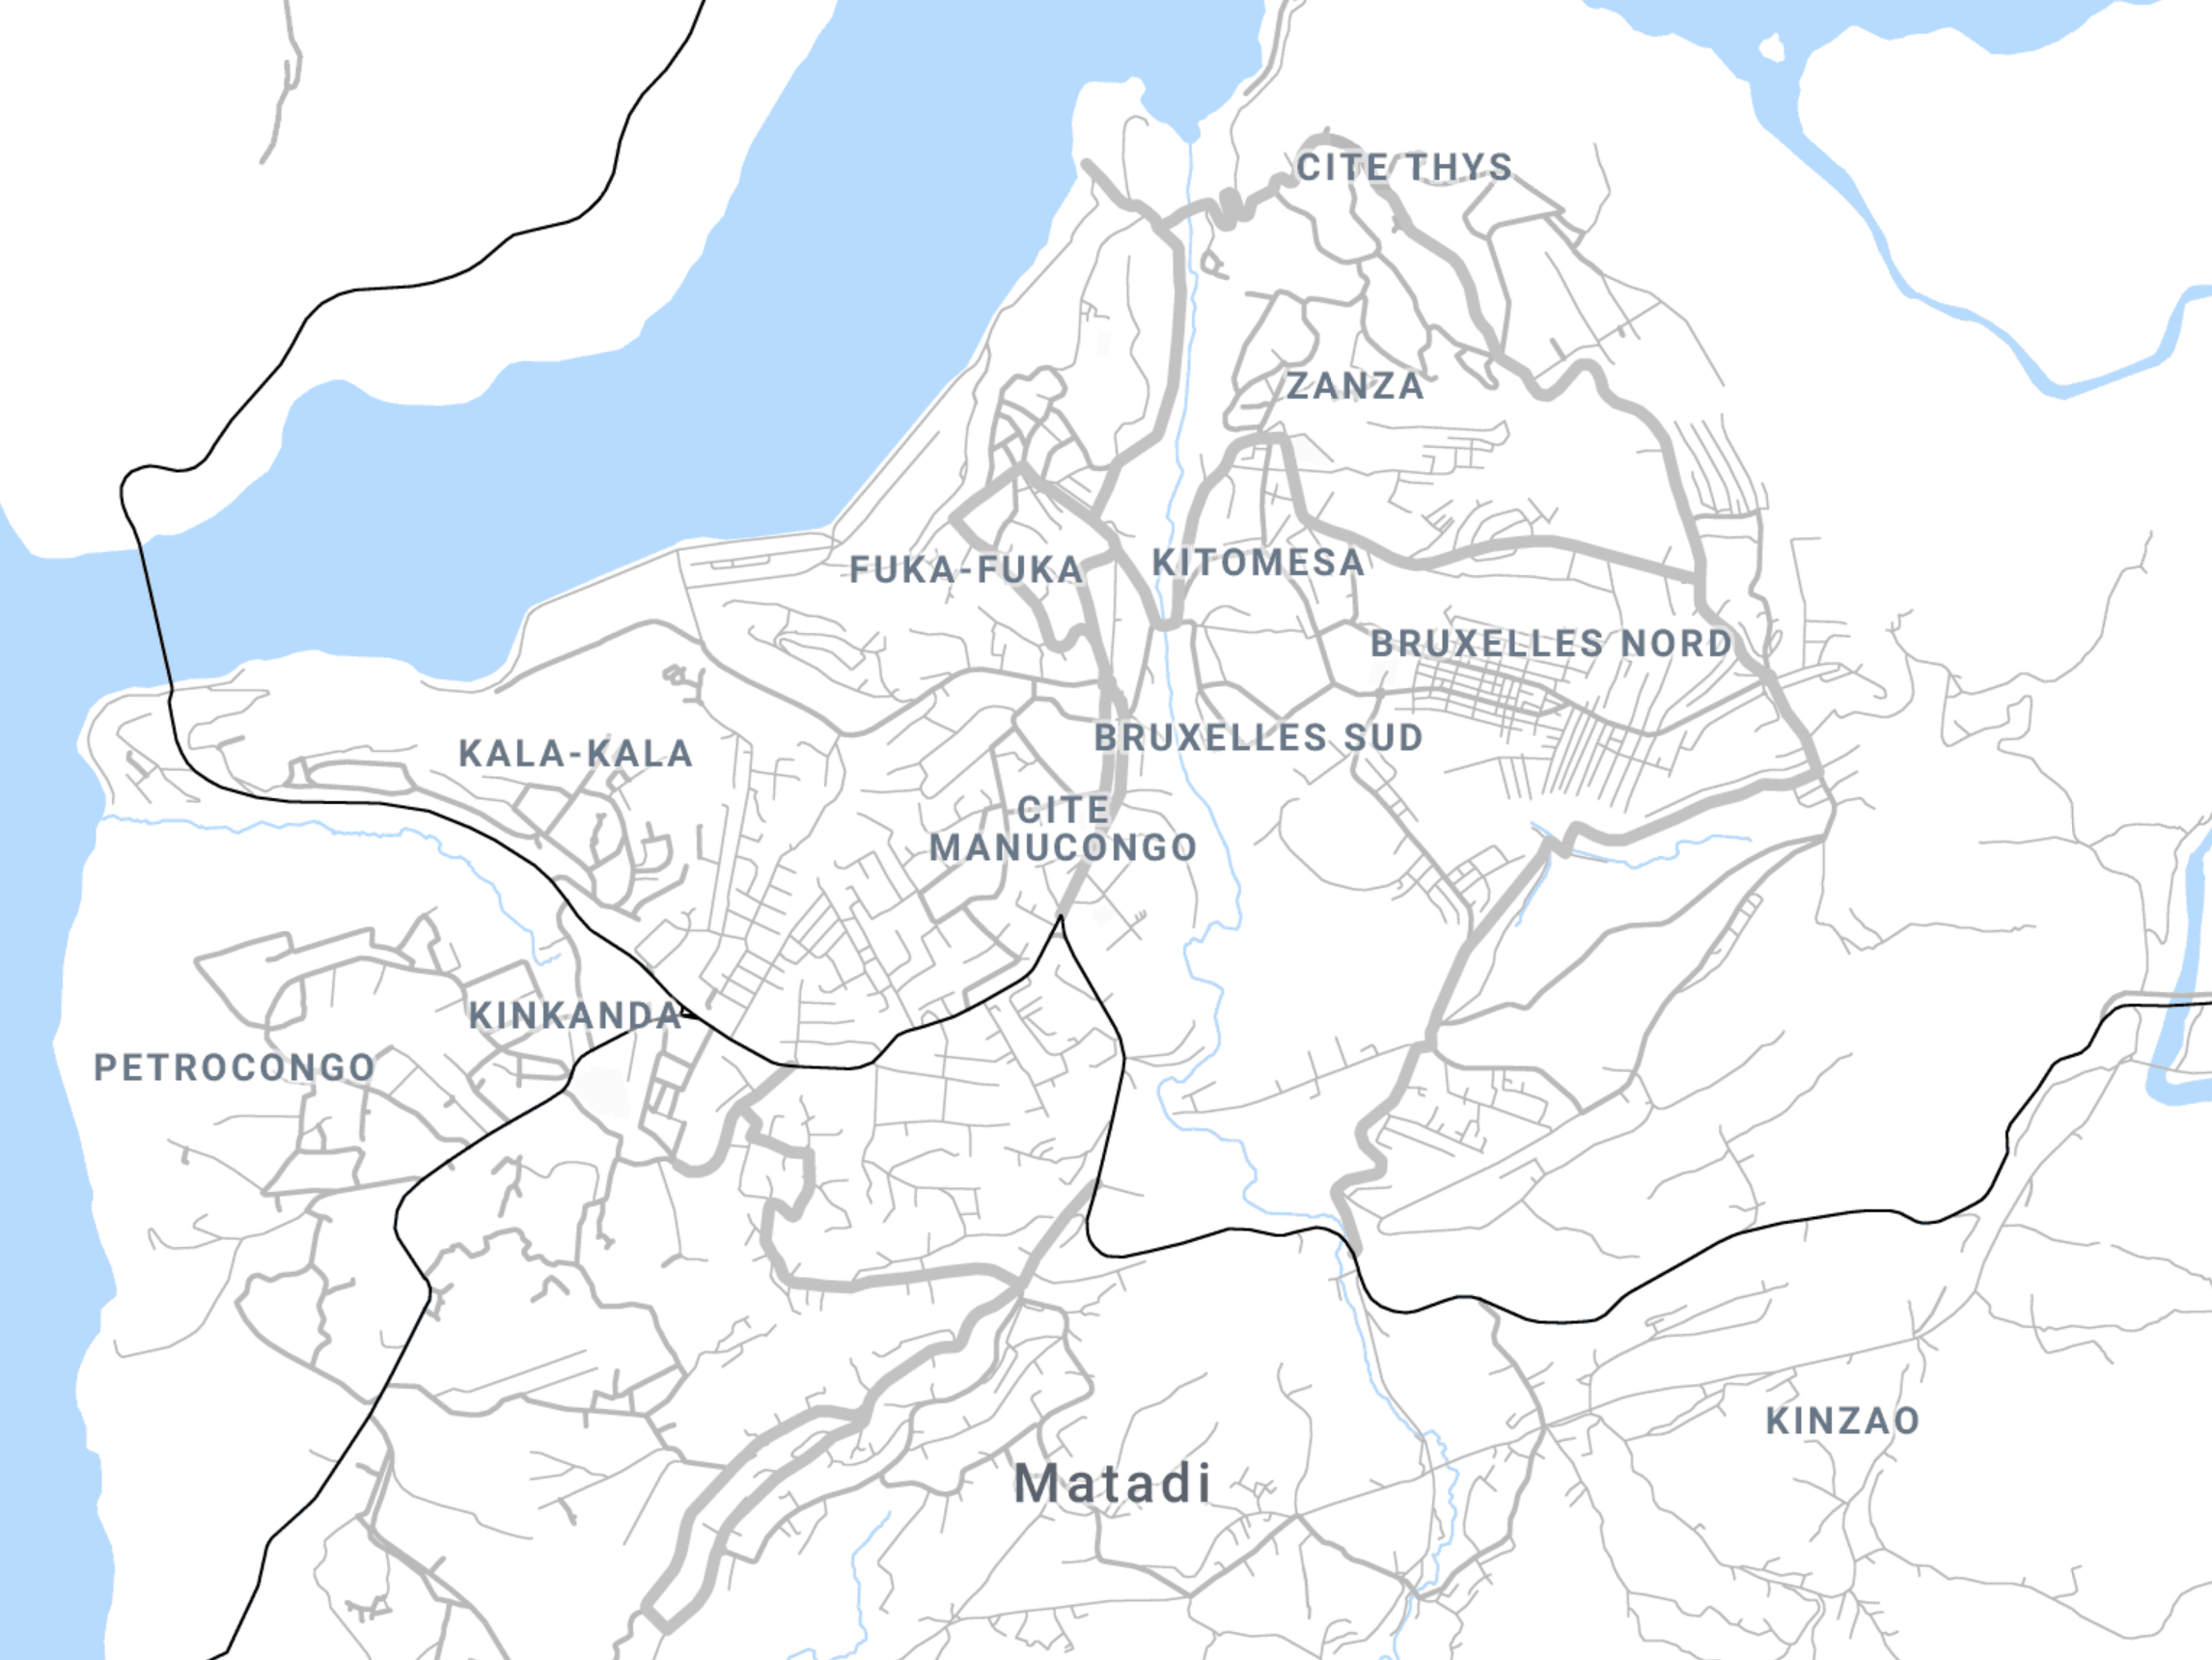
\includegraphics[width=0.8\textwidth]{Figures/matadi.png}
    \caption{Map of Matadi, Democratic Republic of Congo.}
    \label{map:matadi}
\end{figure}

There is insufficient data about the outbreak and specific populations in areas of Matadi, so some assumptions needed to be made. The total population of Matadi in 2005 was 204\,000 \cite{alberti2010reactive}, and a presumed 46\% of this population was under the age of 15 \cite{demographic_dividend}. The total population used for the simulation is thus 93\,840, split between different locations in the city. The network points used for the simulation correspond to the areas labelled on the map in Figure \ref{map:matadi}. The vaccination rate prior to intervention in Matadi was 87.5\% \cite{alberti2010reactive}, and so, the majority of the population was immune to measles. The input data used for the simulation is contained in Table \ref{tab:matadi_input}, where N represents the number of children under 15 in each location, and S represents the number of susceptible children in each location. Since Matadi is a dense city rather than a rural area, the assumptions on travel speeds for a general network do not necessarily apply to this case. Therefore, travel times between locations by road (as obtained from Google Maps) are also used for input, instead of road distances. 

\begin{table}[ht!]
\centering
\resizebox{\textwidth}{!}{%
\begin{tabular}{|c|ccccccccccc|}
\hline
 & \multicolumn{1}{c|}{Urban} & \multicolumn{1}{c|}{x} & \multicolumn{1}{c|}{y} & \multicolumn{1}{c|}{N} & \multicolumn{1}{c|}{S} & \multicolumn{1}{c|}{E} & \multicolumn{1}{c|}{I} & \multicolumn{1}{c|}{V} & \multicolumn{1}{c|}{R} & \multicolumn{1}{c|}{mapX} & mapY \\ \hline
Petrocongo & 0 & -759.07 & 1746.68 & 2000 & 250 & 0 & 0 & 1750 & 0 & -758 & 1747 \\ \cline{1-1}
Cite Thys & 1 & -755.69 & 1751.36 & 3000 & 375 & 0 & 0 & 2625 & 0 & -755 & 1751 \\ \cline{1-1}
Kinzao & 0 & -760.188 & 1753.05 & 1000 & 125 & 0 & 0 & 875 & 0 & -759 & 1752 \\ \cline{1-1}
Bruxelles Sud & 1 & -757.57 & 1750.45 & 15000 & 1875 & 0 & 0 & 13120 & 0 & -758 & 1750 \\ \cline{1-1}
Kala-Kala & 0 & -757.9 & 1748.11 & 4000 & 500 & 0 & 0 & 3500 & 0 & -758 & 1748 \\ \cline{1-1}
Kinkanda & 1 & -758.94 & 1747.98 & 9000 & 1125 & 0 & 0 & 7875 & 0 & -759 & 1748 \\ \cline{1-1}
Cite Manucongo & 1 & -758.004 & 1749.54 & 15000 & 1875 & 0 & 2 & 13120 & 0 & -758 & 1750 \\ \cline{1-1}
Bruxelles Nord & 1 & -757.25 & 1752.478 & 15000 & 1875 & 0 & 0 & 13125 & 0 & -757 & 1752 \\ \cline{1-1}
Fuka-Fuka & 1 & -757.25 & 1749.54 & 10840 & 1355 & 0 & 0 & 9485 & 0 & -757 & 1750 \\ \cline{1-1}
Kitomesa & 1 & -756.86 & 1750.58 & 15000 & 1875 & 0 & 0 & 13125 & 0 & -757 & 1751 \\ \cline{1-1}
Zanza & 1 & -756.47 & 1751.23 & 4000 & 500 & 0 & 0 & 3500 & 0 & -756 & 1751 \\ \hline
\end{tabular}%
}
\caption{Matadi network location details, including populations and coordinates.}
\label{tab:matadi_input}
\end{table}

Since the Matadi network is much smaller and more densely populated than the general network of 160km diameter considered for this project, the frequency of migration needed to be adjusted. Therefore, after adjusting parameters, the amount of migration between any two locations $i$ and $j$ in the Matadi network is $$m_{i,j} = 2 \frac{\sqrt[4]{N_{i} N_{j}}}{\Delta_{i,j}^{2}}.$$ This adjustment reduces the impact that populations have on migration (by setting the exponent of the denominator to $\frac{1}{4}$ instead of $\frac{1}{2})$, to produce more feasible levels of migration for the densely populated network. 

For the simulation of the Matadi outbreak, the death rate is set to 2\% (instead of 10\%), the intervention length to two weeks (instead of four), the number of teams to 18 (instead of 15), and the $R_{0}$ value to 14 (instead of 15). Further, the proportion of a population to be infected before epidemic detection is set to 0.005\% (instead of 0.05\%). All of these parameters are adjusted to mimic the actual results of the outbreak. Figure \ref{res:matadi_valid} shows a comparison of the actual weekly reported measles cases with the average results from over 1000 simulations using this parameter set. The data on the weekly reported measles cases is obtained from Alberti et. al \cite{alberti2010reactive}. The performance of the simulation is easily adjusted according to parameter selection. The team allocation strategy used is population (N), and the vaccine delivery allocation strategy is the number of infectious individuals (I). It is assumed that deliveries are performed by vehicle, since UAVs were not being used for humanitarian aid at the time of the outbreak.

\begin{figure}[ht!]{\textwidth}
    \centering
    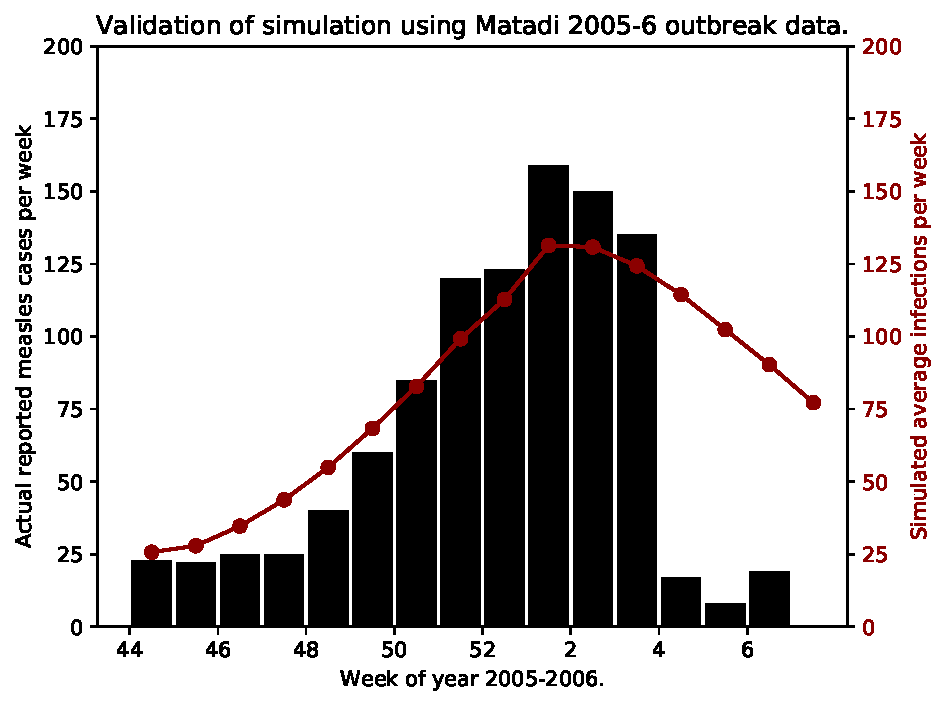
\includegraphics[width=\textwidth, trim={0 0 0 0.67cm},clip]{Matadi_updated.pdf}
    \caption{Comparison of historical measles outbreak results in Matadi with average simulated results.}
    \label{res:matadi_valid}
\end{figure}

The results of the simulation on the Matadi network are similar to the actual outbreak -- an average of 2.26 deaths occurred in simulations (with standard deviation of 1.88), and 9\,315 vaccinations were performed on average (or 71\,884, if previously-vaccinated individuals are re-vaccinated, as was likely the case in the actual intervention). The average progression of the epidemic, as shown in Figure \ref{res:matadi_valid}, is close to the reported outbreak results. It is, however, clear that the intervention in the actual outbreak was significantly more effective and faster than the simulated intervention -- perhaps indicating that teams were able to vaccinate more people daily than in simulations. Using a variable turnout dependant upon the progression of the epidemic, instead of the constant turnout used, would likely produce more accurate results. There are reports of extremely high turnout at vaccination sites for the reported intervention \cite{msf_2006}, and the reported number of weekly infections is not necessarily the same as the number of currently-infected individuals. Thus, these factors can possibly account for the rapid decline in the number of reported infections seen in Figure \ref{res:matadi_valid}, when compared to simulations.

The results of this test for validity of the simulation model indicate that the model is indeed valid, since it can reproduce historical epidemics fairly accurately. The model would likely be even more accurate if more detailed data could be used as input, and parameters could be more finely tuned. Furthermore, the model is consistent -- the standard deviation of results is relatively low. It can therefore be concluded that the model is valid and results produced are likely to be reliable.